\section{Results}

This section shows the results of the environment model and the I2A implementation. And shows the performance of I2A over the model-free baseline and the copy model.

%In the following the performance of I2A over the model-free baseline and the copy model is shown. Also the predicted rollouts of the environment model.

\subsection{Environment Model Training}

The trained environment model is a imperfect model which is in most cases able to predict a few steps into the future, but it is bad in predicting far into the future.\\

\begin{figure}[H] 
  \centering   
  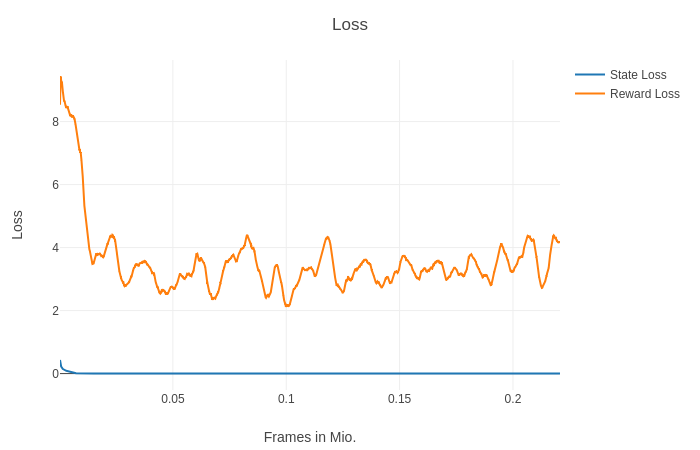
\includegraphics[width=0.9\columnwidth]{./Images/hunt_environment_model_loss.png}
  \caption{Environment model loss curve} 
  \label{fig:env_model_loss} 
\end{figure} 

The figure \ref{fig:env_model_loss} show the loss curve of the environment model training. It seems as if the loss stagnates very soon, but the main advantage in correct predictions is learned in the part with small loss changes. To learn the general structure of the maze is easy but to predict the correct position of the player and the ghosts is really hard, but has only a small impact on the loss.


\begin{figure}[H] 
  \centering   
  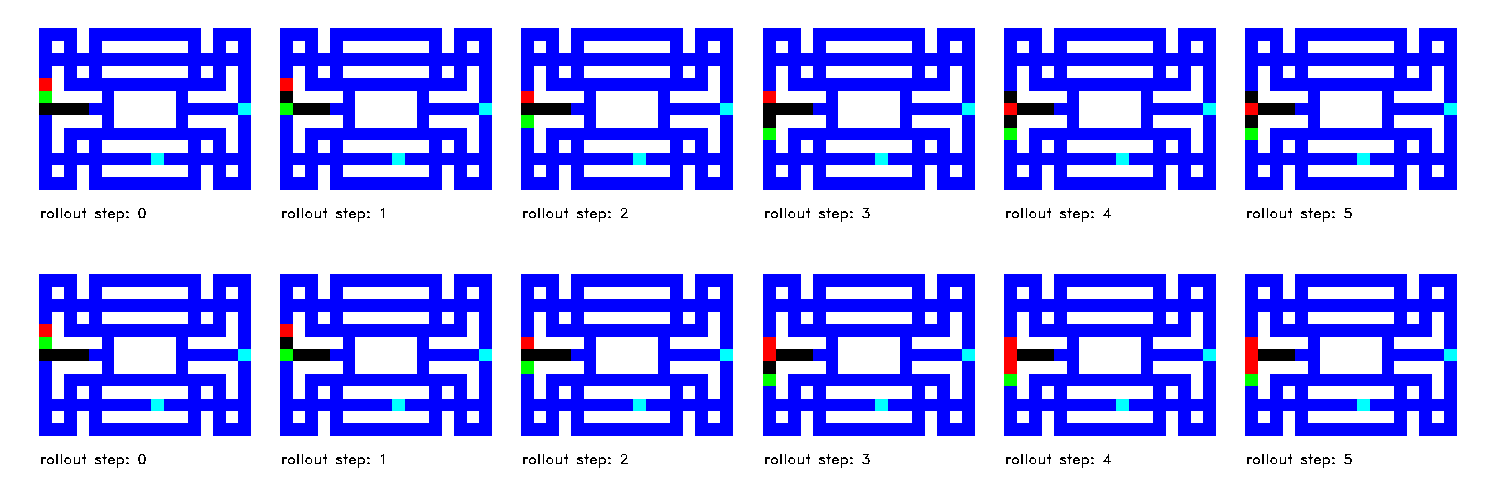
\includegraphics[width=\columnwidth]{./Images/env_model_rollouts.png}
  \caption{Environment model rollouts, top true observation, bottom predicted observation, rollouts steps from left to right} 
  \label{fig:environment_model_rollouts} 
\end{figure} 



Figure \ref{fig:environment_model_rollouts} shows the true next observation in the upper row and the predicted observation in the lower row. From left to right it shows the rollout steps, the prediction is always based on the previouse rollout step. In the beginning the prediction is quite good but the errors accumulate, leading to prediction errors like the one in rollout step 3 of figure \ref{fig:environment_model_rollouts}. The environment model is unsure where the ghost, the red points, are moving and as a result it predicts the ghost at two positions.



\subsection{I2A MiniPacman Results}


To compare the performance, we trained MiniPacman Hunt with a A2C model-free baseline, the copy model and I2A agent.\\


TODO regular results.\\
\begin{figure}[H] 
  \centering   
  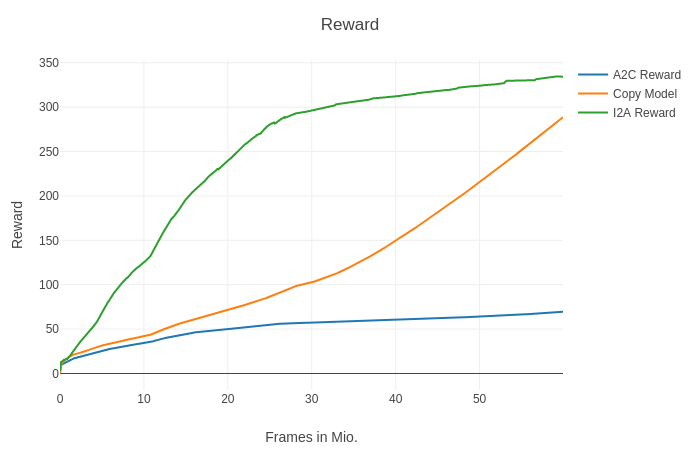
\includegraphics[width=0.9\columnwidth]{./Images/regular_rewards_compare.png}
  \caption{Reached rewards on the environment MiniPacman Hunt. Green curve I2A run with 2 rollouts, blue curve model-free A2C baseline and orange curve copy model results.} 
  \label{fig:mini_pacman_hunt_rewards} 
\end{figure} 

The results of the trained agents on MiniPacman in Hunt mode are shown in figure \ref{fig:mini_pacman_hunt_rewards}. As you can see the I2A algorithm outperform A2C and the Copy model.


\begin{figure}[H] 
  \centering   
  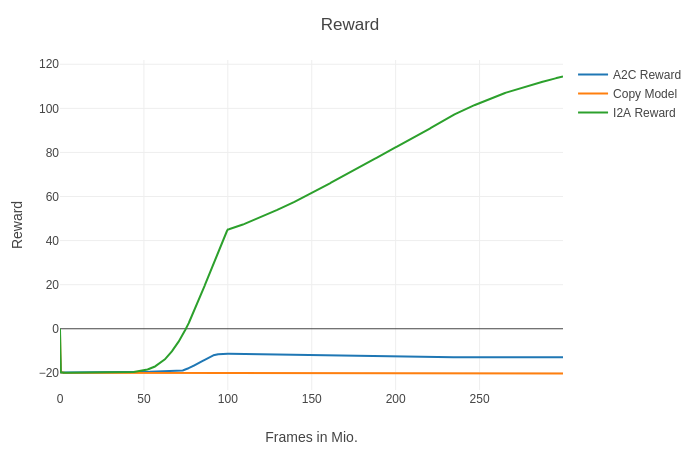
\includegraphics[width=0.9\columnwidth]{./Images/hunt_rewards_compare.png}
  \caption{Reached rewards on the environment MiniPacman Hunt. Green curve I2A run with 2 rollouts, blue curve model-free A2C baseline and orange curve copy model results.} 
  \label{fig:mini_pacman_hunt_rewards} 
\end{figure} 

TODO compare result with the one of the i2a paper.